\documentclass{beamer}
%\documentclass[aspectratio=169]{beamer}
\usepackage{ctex,hyperref}
\usepackage[T1]{fontenc}
\usepackage{latexsym,amsmath,xcolor,multicol,booktabs,calligra,array}
\usepackage{graphicx,pstricks,listings,stackengine}

\title{Cell-Free Massive MIMO Channel Prediction}
\subtitle{Literature-Grounded Study with Baseline and Ablation Analysis}
\author[Bhadresh L | Pavan Kumar M | Parth Pandey]{Bhadresh L (CS23I1014) \and Pavan Kumar M (CS23B2029) \and Parth Pandey (CS23I1064)}
\institute[IIITDM Kancheepuram]{IIITDM Kancheepuram, COM523 Wireless Networks}
\date{April 2026}
\usepackage{CNU}

% Ensure title-page identity text is visible on light backgrounds.
\setbeamercolor{author}{fg=black,bg=white}
\setbeamercolor{institute}{fg=black,bg=white}
\setbeamercolor{date}{fg=black,bg=white}

% Keep footer identity text inside blue footer bars on all slides.
\setbeamercolor{author in head/foot}{fg=white,bg=CNU}
\setbeamercolor{institute in head/foot}{fg=white,bg=CNU}
\setbeamercolor{title in head/foot}{fg=white,bg=CNU}

% Keep progress/header bar labels fully visible.
\setbeamerfont{section in head/foot}{size=\tiny}
\setbeamerfont{subsection in head/foot}{size=\tiny}

% Compact table spacing and enforce in-frame width fitting.
\setlength{\tabcolsep}{4pt}
\renewcommand{\arraystretch}{1.1}

\begin{document}

\kaishu
\begin{frame}
    \titlepage
    \begin{figure}[htpb]
        \begin{center}
            
\includegraphics[width=0.26\linewidth]{pic/首师大logo.png}
        \end{center}
    \end{figure}
\end{frame}

\begin{frame}{Presentation Roadmap}
    \tableofcontents[sectionstyle=show,subsectionstyle=show/shaded/hide,subsubsectionstyle=show/shaded/hide]
\end{frame}

\section[Lit + Motivation]{Literature Survey and Motivation}

\begin{frame}{Literature Survey: Key Takeaways}
    \footnotesize
    \begin{itemize}
        \item Massive MIMO and Cell-Free MIMO improve coverage, but CSI aging degrades beamforming under mobility.
        \item Classical predictors (AR, Kalman/VKF) are interpretable and strong baselines, but can be computationally heavy.
        \item Recent DL methods (CNN, LSTM, Transformer) improve prediction accuracy in dynamic channels.
        \item Literature survey highlights a gap: lightweight predictors for \textbf{distributed, irregular AP topologies} in Cell-Free systems.
        \item Our project targets this gap with a temporal CNN and a GNN-CNN hybrid, tested against AR and VKF baselines.
    \end{itemize}
\end{frame}

\begin{frame}{Motivation and Research Question}
    \small
    \textbf{Motivation from literature survey and report:}
    \begin{itemize}
        \item Channel estimates become stale during pilot-to-data delay, especially at high velocity.
        \item Centralized methods are accurate but can add latency and scale poorly.
        \item Edge-ready 6G systems need low-latency prediction with strong robustness.
    \end{itemize}

    \vspace{0.3em}
    \textbf{Research question:}
    \begin{block}{ }
    Can a decentralized temporal model outperform both classical predictors and centralized graph aggregation for multi-step channel prediction in Cell-Free Massive MIMO?
    \end{block}
\end{frame}

\section{Initial Understanding}

\begin{frame}{Our Initial Understanding (from notebooks + early report)}
    \footnotesize
    \begin{itemize}
        \item Initial hypothesis: neighboring APs should share useful correlation, so GNN aggregation should help prediction.
        \item Early pipeline in notebooks: dataset generation, train CNN-only and GNN-CNN, evaluate by velocity, step, ablations, and efficiency.
        \item System configuration used across experiments: $L=16$ APs, $N=4$ antennas/AP, $K=4$ UEs, history $T_h=10$, horizon $T_p=3$.
        \item Velocity settings: 30, 60, 120 km/h; layouts: random and grid.
        \item Key insight that changed trajectory: normalization and physically grounded channel generation strongly impact model behavior.
    \end{itemize}
\end{frame}

\section{Baselines}

\begin{frame}{Baseline 1: AR Predictor}
    \small
    \begin{itemize}
        \item Scalar AR(4) per channel coefficient using Yule-Walker estimation.
        \item Predicts future values autoregressively from local history only.
        \item Strength: simple, low parameterization, easy to interpret.
        \item Limitation: weak under non-stationary/high-mobility channel evolution.
    \end{itemize}
\end{frame}

\begin{frame}{Baseline 2: Vector Kalman Filter (VKF)}
    \small
    \begin{itemize}
        \item Joint state tracking across AP antenna dimensions with covariance updates.
        \item Uses linear state-space prediction/correction and matrix inversions.
        \item Strength: principled statistical tracker with good physical interpretability.
        \item Limitation: computational overhead and sensitivity to model mismatch.
    \end{itemize}
\end{frame}

\begin{frame}{Baseline Summary Table}
    \scriptsize
    \centering
    \resizebox{\linewidth}{!}{%
    \begin{tabular}{p{2.1cm}p{3.1cm}p{3.4cm}p{2.6cm}}
        \toprule
        Method & Core idea & Strength & Practical limitation \\
        \midrule
        AR(4) & Per-link autoregression from recent history & Very lightweight and fast to deploy & Misses richer temporal/spatial structure \\
        VKF & Joint vector state prediction with covariance update & Strong classical benchmark and interpretable & High latency due to matrix operations \\
        \bottomrule
    \end{tabular}%
    }
\end{frame}

\section[Approaches + Experiments]{Our Approaches and Experiments}

\begin{frame}{Approach 1: CNN-Only (Decentralized)}
    \small
    \begin{itemize}
        \item Shared temporal Conv1D stack per AP, followed by prediction head.
        \item Per-AP normalization and de-normalization in forward pass.
        \item No AP-to-AP message passing: purely local temporal representation learning.
        \item Designed for low-latency decentralized deployment.
    \end{itemize}
\end{frame}

\begin{frame}{Approach 2: GNN-CNN (Centralized Aggregation)}
    \small
    \begin{itemize}
        \item Stage 1: local temporal CNN embedding per AP.
        \item Stage 2: single GCN layer over KNN AP graph ($k=3$) to aggregate neighborhood context.
        \item Stage 3: prediction head for multi-step channel output.
        \item Goal: test whether explicit spatial aggregation improves prediction under mobility.
    \end{itemize}
\end{frame}

\begin{frame}{All Experimentations Performed}
    \scriptsize
    \centering
    \resizebox{\linewidth}{!}{%
    \begin{tabular}{p{1.2cm}p{2.7cm}p{5.8cm}}
        \toprule
        Exp. & Name & Objective \\
        \midrule
        1 & NMSE vs velocity & Compare AR, VKF, CNN-Only, GNN-CNN at 30/60/120 km/h \\
        2 & NMSE vs step & Evaluate error growth for $k=1,2,3$ ahead prediction \\
        3 & GCN ablation & Compare CNN-Only vs GNN-CNN directly \\
        4 & Topology ablation & Compare random vs grid AP layout impact \\
        5 & Efficiency & Compare parameters and inference latency \\
        \bottomrule
    \end{tabular}%
    }

    \vspace{0.5em}
    \begin{itemize}
        \item Iteration progression used in report: initial model $\rightarrow$ normalization fix $\rightarrow$ GBSM + VKF verification.
    \end{itemize}
\end{frame}

\begin{frame}{Result Plot: NMSE vs Velocity (Random Layout)}
    \centering
    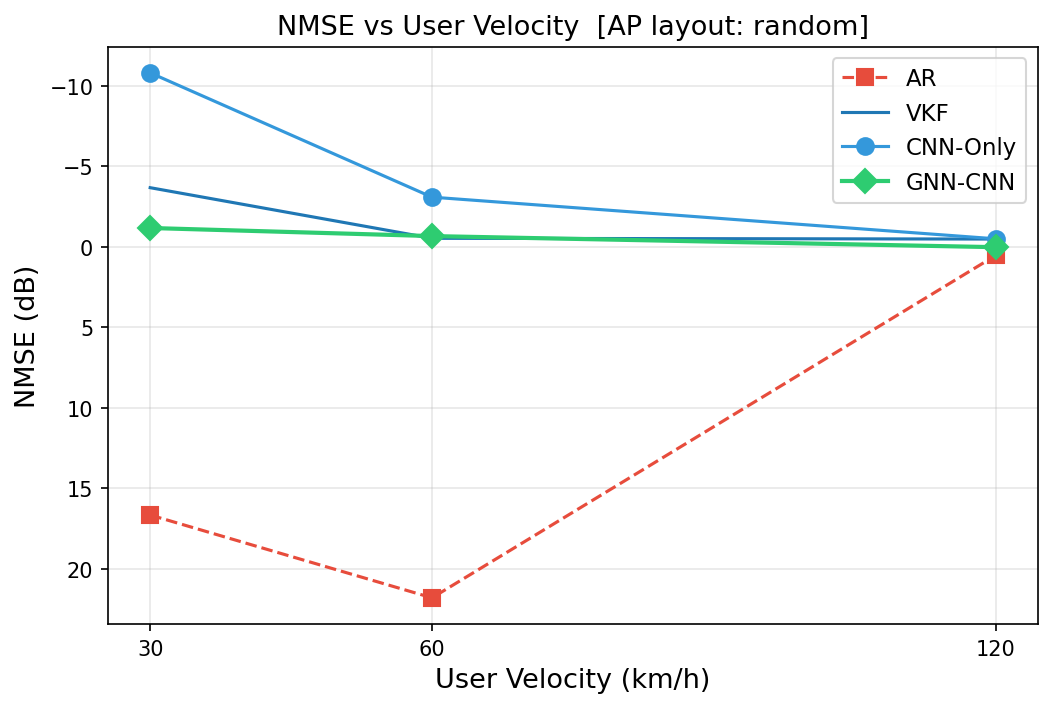
\includegraphics[width=0.82\linewidth]{../cell_free_channel_prediction/kaggle_working_backup_last/results/fig1_nmse_vs_velocity_random.png}
\end{frame}

\begin{frame}{Result Plot: NMSE vs Velocity (Grid Layout)}
    \centering
    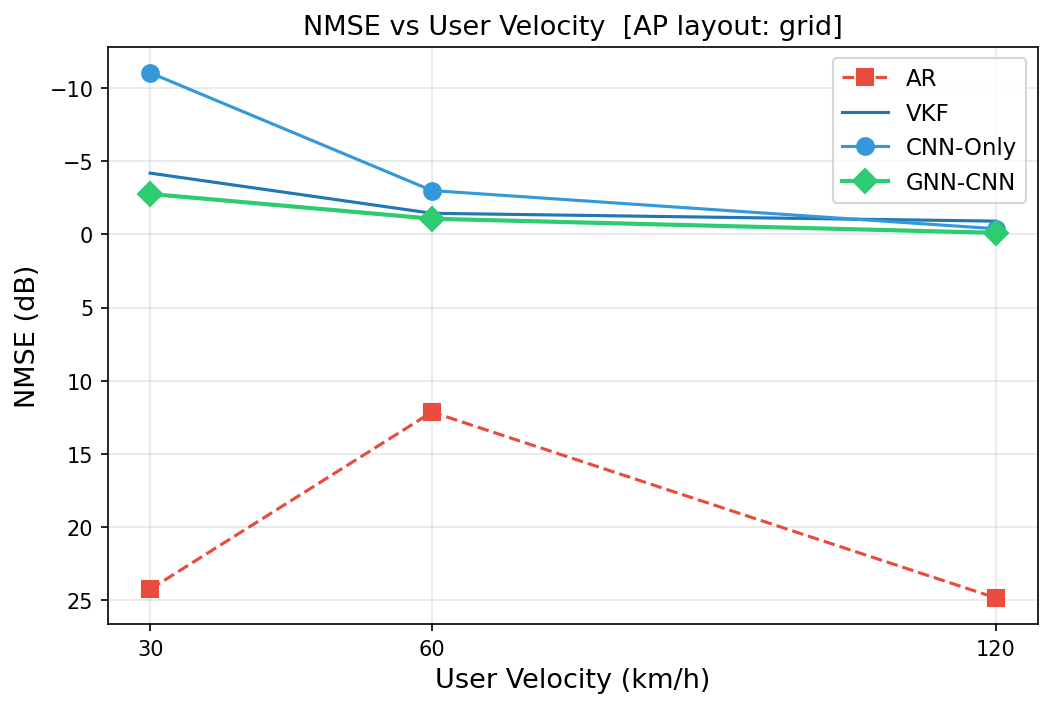
\includegraphics[width=0.82\linewidth]{../cell_free_channel_prediction/kaggle_working_backup_last/results/fig1_nmse_vs_velocity_grid.png}
\end{frame}

\begin{frame}{Result Plot: NMSE vs Prediction Step}
    \begin{columns}[T]
        \column{0.49\linewidth}
        \centering
        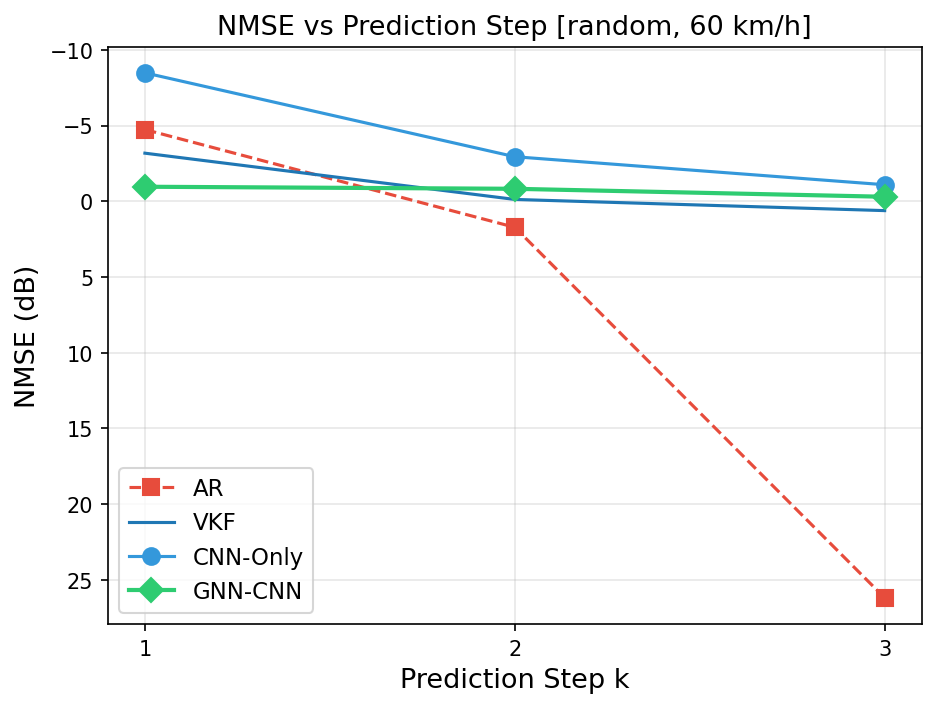
\includegraphics[width=\linewidth]{../cell_free_channel_prediction/kaggle_working_backup_last/results/fig2_nmse_vs_step_random_60.png}
        {\tiny 60 km/h (random)}

        \column{0.49\linewidth}
        \centering
        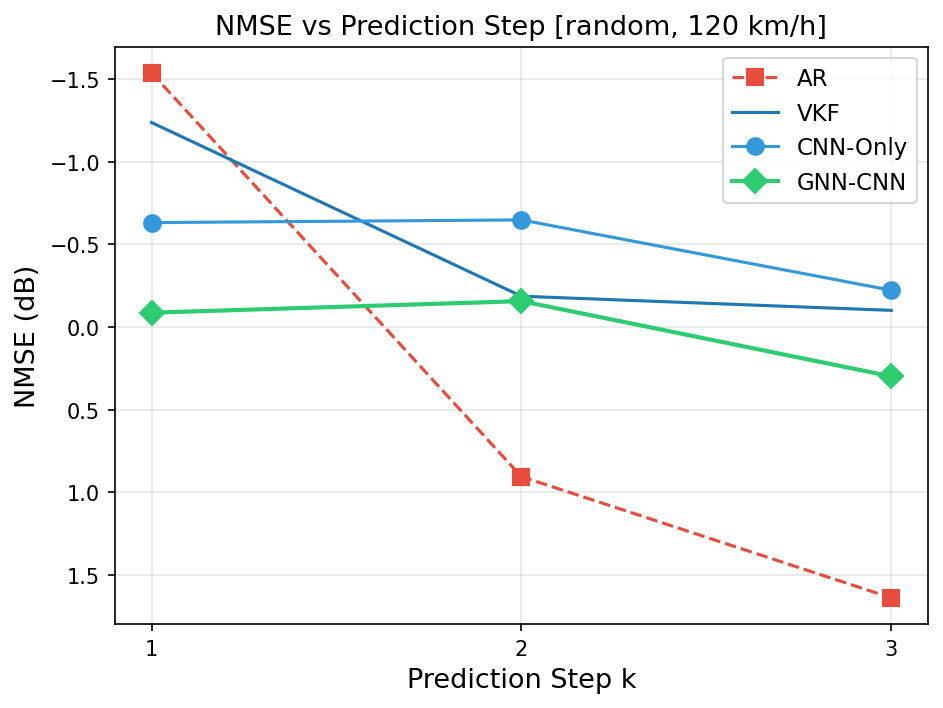
\includegraphics[width=\linewidth]{../cell_free_channel_prediction/kaggle_working_backup_last/results/fig2_nmse_vs_step_random_120.png}
        {\tiny 120 km/h (random)}
    \end{columns}
\end{frame}

\begin{frame}{Result Plot: GCN Ablation and Topology Ablation}
    \begin{columns}[T,onlytextwidth]
        \column{0.49\linewidth}
        \centering
        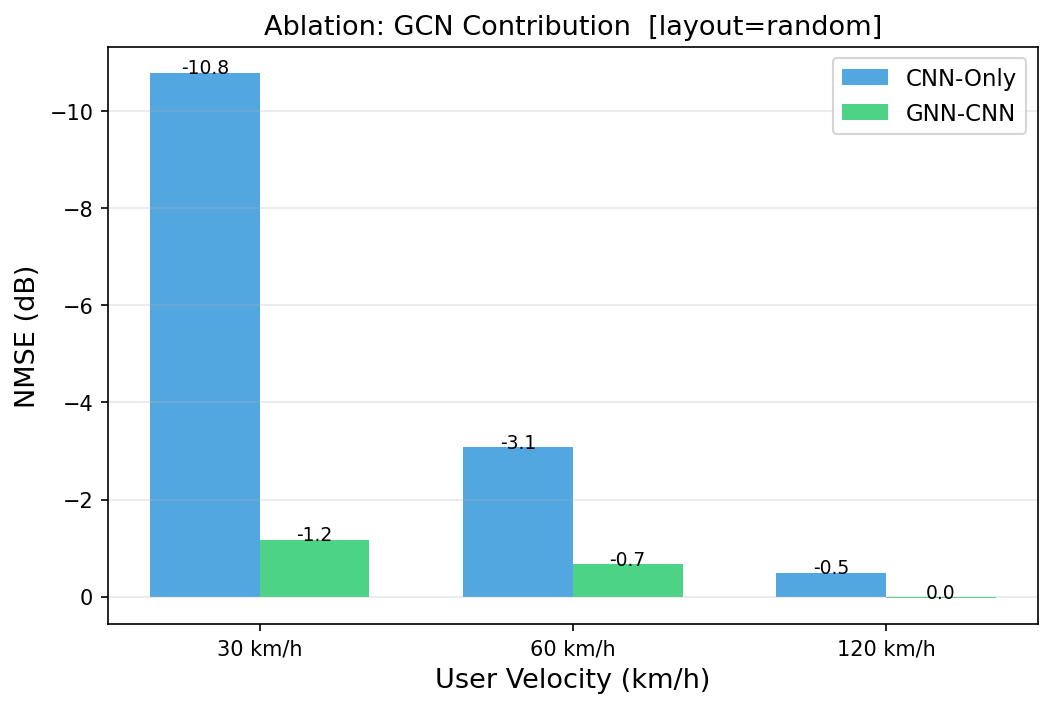
\includegraphics[width=\linewidth,height=0.56\textheight,keepaspectratio]{../cell_free_channel_prediction/kaggle_working_backup_last/results/fig3_ablation_gcn_random.png}
        {\tiny CNN-Only vs GNN-CNN}

        \column{0.49\linewidth}
        \centering
        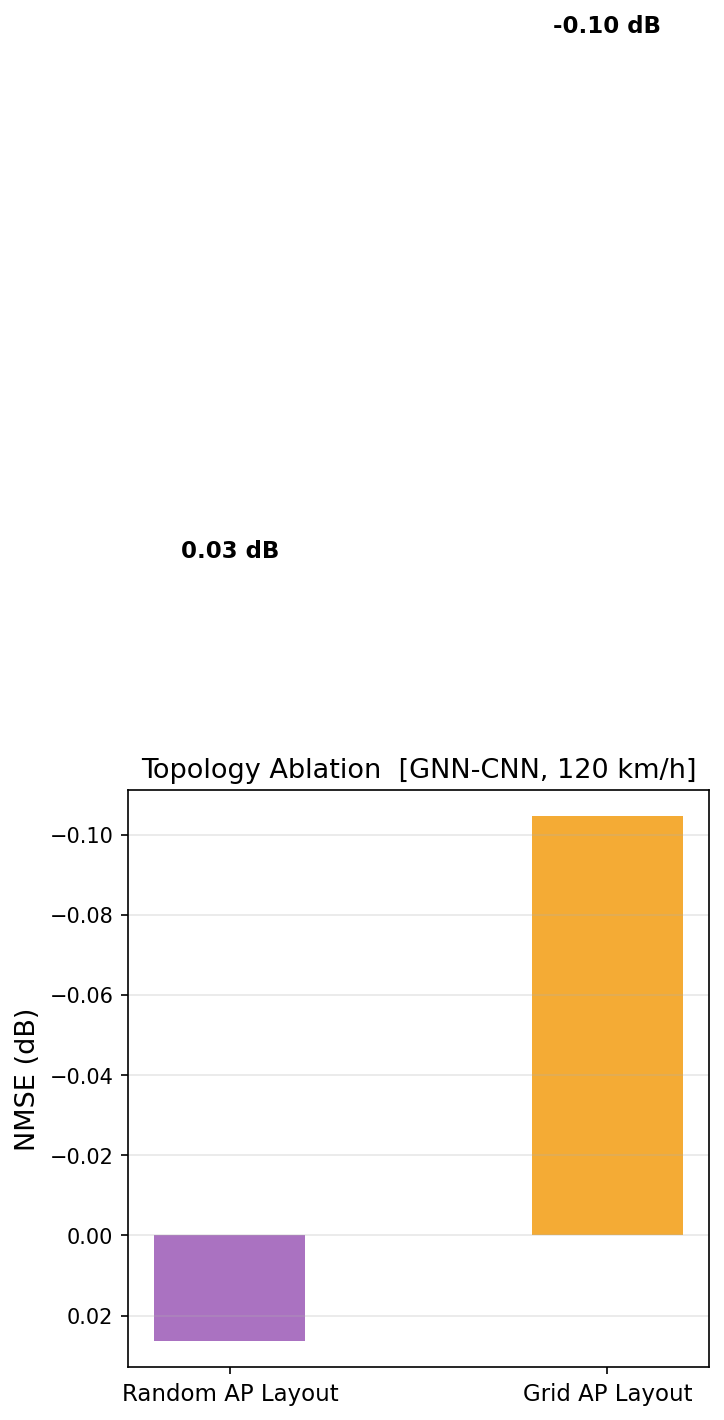
\includegraphics[width=\linewidth,height=0.56\textheight,keepaspectratio]{../cell_free_channel_prediction/kaggle_working_backup_last/results/fig4_ablation_topology_120.png}
        {\tiny Grid vs random (120 km/h)}
    \end{columns}
\end{frame}

\section[Baseline Comparison]{Comparison with Baselines}

\begin{frame}{Comparison Table: NMSE vs Velocity (Random Layout)}
    \scriptsize
    \centering
    \resizebox{0.9\linewidth}{!}{%
    \begin{tabular}{lccc}
        \toprule
        Method & 30 km/h & 60 km/h & 120 km/h \\
        \midrule
        AR & 16.65 & 21.79 & 0.54 \\
        VKF & -3.67 & -0.52 & -0.48 \\
        CNN-Only & \textbf{-10.79} & \textbf{-3.08} & \textbf{-0.49} \\
        GNN-CNN & -1.16 & -0.66 & 0.03 \\
        \bottomrule
    \end{tabular}%
    }

    \vspace{0.4em}
    \small More negative NMSE is better.
\end{frame}

\begin{frame}{Comparison Table: NMSE vs Velocity (Grid Layout)}
    \scriptsize
    \centering
    \resizebox{0.9\linewidth}{!}{%
    \begin{tabular}{lccc}
        \toprule
        Method & 30 km/h & 60 km/h & 120 km/h \\
        \midrule
        AR & 24.26 & 12.15 & 24.84 \\
        VKF & -4.19 & -1.44 & -0.90 \\
        CNN-Only & \textbf{-11.04} & \textbf{-2.99} & -0.39 \\
        GNN-CNN & -2.76 & -1.07 & \textbf{-0.10} \\
        \bottomrule
    \end{tabular}%
    }
\end{frame}

\begin{frame}{Efficiency Table: Practical Deployment View}
    \scriptsize
    \centering
    \resizebox{0.9\linewidth}{!}{%
    \begin{tabular}{lccc}
        \toprule
        Method & Params & Mean latency (ms) & Std (ms) \\
        \midrule
        GNN-CNN & 51008 & 0.928 & 0.146 \\
        CNN-Only & 46848 & \textbf{0.712} & 0.038 \\
        AR & 1024 & 9.639 & 0.359 \\
        VKF & 256 & 35.972 & 1.037 \\
        \bottomrule
    \end{tabular}%
    }
\end{frame}

\section[Result Insights]{Understanding of Results}

\begin{frame}{Understanding the Results}
    \small
    \begin{itemize}
        \item CNN-Only consistently beats VKF and often beats GNN-CNN, especially at 30/60 km/h.
        \item Per-AP normalization was the turning point; without it, neural models underperformed.
        \item GNN aggregation can mix uncorrelated AP innovations, hurting prediction in some settings.
        \item Grid layout slightly helps GNN-CNN at very high speed (120 km/h), indicating topology still matters.
        \item For edge deployment, CNN-Only gives the best overall accuracy-latency trade-off.
    \end{itemize}
\end{frame}

\section{Conclusion}

\begin{frame}{Conclusion}
    \small
    \begin{itemize}
        \item We started with a centralized-correlation hypothesis (GNN-CNN expected to win).
        \item Through iterative experimentation (modeling fixes, normalization, GBSM, VKF benchmark), we observed the opposite.
        \item A decentralized temporal CNN achieved the strongest and most stable performance.
        \item Final takeaway: for this project setting, local temporal learning is more effective and more deployable than heavier centralized aggregation.
    \end{itemize}
\end{frame}

\section[References]{References (from Literature Survey)}

\begin{frame}[allowframebreaks]{References}
    \scriptsize
    \begin{thebibliography}{99}
        \bibitem{ngo2017} H. Q. Ngo et al., ``Cell-Free Massive MIMO Versus Small Cells,'' IEEE TWC, 2017.
        \bibitem{elhoushy2022} S. Elhoushy et al., ``Cell-Free Massive MIMO: A Survey,'' IEEE Communications Surveys \& Tutorials, 2022.
        \bibitem{zheng2021} J. Zheng et al., ``Impact of Channel Aging on Cell-Free Massive MIMO over Spatially Correlated Channels,'' IEEE TWC, 2021.
        \bibitem{kim2021} H. Kim et al., ``Massive MIMO Channel Prediction: Kalman Filtering vs. Machine Learning,'' IEEE Transactions on Communications, 2021.
        \bibitem{jiang2022} H. Jiang et al., ``Accurate Channel Prediction Based on Transformer,'' IEEE JSAC, 2022.
        \bibitem{wang2024} Z. Wang et al., ``A Tutorial on Extremely Large-Scale MIMO for 6G,'' IEEE Communications Surveys \& Tutorials, 2024.
        \bibitem{li2025} B. Li et al., ``A Survey of AI Enabled Channel Estimation Methods,'' Artificial Intelligence Review, 2025.
    \end{thebibliography}
\end{frame}

\begin{frame}
    \begin{center}
        {\Huge\calligra Thank You}
    \end{center}
\end{frame}

\end{document}